% Chinese reading edition; scientific content follows main.tex.
\documentclass[10pt,twocolumn,letterpaper]{article}
\usepackage[review]{cvpr}
\usepackage{graphicx}
\usepackage{amsmath,amssymb}
\usepackage{booktabs}
\usepackage{tabularx}
\usepackage{microtype}
\usepackage{xcolor}
\newcommand{\method}{FewClick}
\newcommand{\blankfield}{\rule{0.7\linewidth}{0.4pt}}
% Only the experimental artwork/tables are reserved; numerical prose is retained.
\newcommand{\reserved}[2]{\fbox{\begin{minipage}[c][#1][c]{\dimexpr\linewidth-2\fboxsep-2\fboxrule\relax}\centering\small\color{gray}#2\end{minipage}}}
\newcommand{\tableplaceholder}[3]{\begin{table}[t]\centering\caption{#2}\label{#1}\reserved{#3}{Experimental table reserved}\end{table}}

\usepackage{xeCJK}
\setCJKmainfont{Noto Serif CJK SC}[BoldFont={Noto Sans CJK SC},ItalicFont={Noto Serif CJK SC}]
\setCJKsansfont{Noto Sans CJK SC}
\setCJKmonofont{Noto Sans Mono CJK SC}
\definecolor{cvprblue}{rgb}{0.21,0.49,0.74}
\usepackage[pagebackref,breaklinks,colorlinks,allcolors=cvprblue]{hyperref}
\def\confName{CVPR}
\def\confYear{2027}
\renewcommand{\figurename}{图}
\renewcommand{\tablename}{表}
\renewcommand{\refname}{参考文献}
\patchcmd{\abstract}{Abstract}{摘要}{}{\errmessage{Cannot translate abstract heading}}
\patchcmd{\abstract}{\it\ignorespaces}{\normalfont\ignorespaces}{}{}
\title{FewClick：面向用户指定病理组织分割的\\少量点击交互框架}
\author{CVPR匿名投稿}
\begin{document}
\maketitle
\begin{abstract}
全切片图像（WSIs）中的组织分割可用于组织定量与肿瘤微环境分析。固定类别模型难以直接适应用户指定的目标，而对每个不连通区域分别添加提示又会增加交互负担。本文提出FewClick，通过在一个支持图像块中提供少量正负点击，将所定义的组织目标传播至同一切片的各区域，查询区域无需额外人工提示。FewClick结合多尺度整块／分块特征与正负支持证据，识别目标并区分非目标组织。模型通过由粗到细的密集对应关系迁移预测的支持区域概率，细化查询掩码，并利用区域上下文组织不同尺度的组织结构。对于每个“切片—目标”组合，仅在一个支持图像块上提供三个正点击和两个负点击，FewClick便在15张WSI、152个组织任务上取得43.75\%的整片宏平均Dice和40.98\%的严格远端宏平均Dice。在新增适配预算匹配的条件下，两项指标分别比SANSA高10.52和10.86个百分点。在11,000个同片远端开发任务上，FewClick将目标缺失时的误报面积比例从SANSA的14.79\%降至7.75\%，下降7.04个百分点。同时，FewClick在包含目标的查询区域上保持了与SANSA相当的分割精度。
\end{abstract}

\section{引言}
全切片图像（WSIs）以高分辨率记录大范围组织形态，可用于肿瘤测量、组织组成分析与感兴趣区域选择。HistoSegNet和CAMEL等弱监督组织分割方法降低了标注需求，但预测的仍是预先定义的组织类别~\cite{chan2019histosegnet,xu2019camel}。复杂的组织边界与显著的尺度变化使密集像素标注成本高昂。此外，分割目标会随研究需求变化：同一张切片可能需要分别提取肿瘤上皮、间质或脂肪组织。固定的分割输出通道无法直接表达这种由用户定义的目标。

基于点击的交互方法与可提示基础模型提供了直接指定分割目标的方式~\cite{sofiiuk2022ritm,liu2023simpleclick,kirillov2023sam}。但将其应用于整张WSI仍面临三个挑战。首先，同一种组织可能分布于多个不连通区域，因此局部提示需要将信息传递至其邻域之外。其次，不同组织可能具有相似的局部外观，目标识别因而依赖周围的组织结构以及应予排除的示例。第三，组织识别需要较大范围的上下文，而小结构的轮廓描绘需要局部细节~\cite{tokunaga2019awmf,vanrijthoven2021hooknet,ho2021dmmn}。在整片尺度上，重复添加提示和重复进行图像计算进一步加重了这些问题。

因此，少量点击驱动的WSI分割需要在空间分离的区域中找回目标，同时限制目标缺失区域中的误检。当一个支持示例引导整张切片的预测时，目标覆盖与误检之间的权衡尤为关键。FewClick结合正负支持证据与密集概率迁移来处理这两方面需求。整块与分块特征保留组织结构及局部细节，多尺度区域上下文辅助目标识别，对应关系则将支持证据关联至远端查询位置。

图~\ref{fig:overview}概述了FewClick。共享骨干网络编码对齐的精细、中间和粗尺度视野，并融合整块与分块精细特征。区域池化与跨尺度消息组织上下文信息。正负支持点击引导初始预测，随后由粗到细的对应关系迁移预测的支持区域概率，细化查询logits。同一支持示例用于整片预测，无需追加人工提示。

本文的贡献包括三个方面。(1) 提出整片组织传播框架，仅需在一个支持图像块中提供少量正负点击，查询区域无需追加人工提示。(2) 结合多尺度整块／分块特征、正负支持证据与由粗到细的概率迁移，兼顾目标覆盖与非目标排除，并利用区域上下文组织空间信息。(3) 在共同的支持提示与新增适配预算下，基于15张WSI和11,000个远端开发任务比较六种方法，并通过匹配对照量化覆盖–误检权衡。FewClick在所比较的方法中取得最高的整片宏平均Dice（43.75\%），比SANSA高10.52个百分点。在远端开发队列上，其目标缺失FPA最低（7.75\%），同时保持最高的目标存在宏平均Dice（42.11\%）。

\section{相关工作}
\paragraph{组织分割与多尺度表征。}
HistoSegNet从图像块级标签生成组织掩码，CAMEL则通过多实例标签扩充完成组织病理分割~\cite{chan2019histosegnet,xu2019camel}。AWMF-CNN对不同视野进行自适应加权，HookNet连接同心的不同分辨率分支，DMMN融合多个放大倍率进行组织分割~\cite{tokunaga2019awmf,vanrijthoven2021hooknet,ho2021dmmn}。这些方法表明，组织形态及其周围结构均具有重要作用。HIPT为吉像素切片级任务学习层级表征~\cite{chen2022hipt}。CTransPath和UNI通过自监督预训练提供可迁移的病理编码器~\cite{wang2022ctranspath,chen2024uni}；Phikon-v2采用基于DINOv2的训练~\cite{filiot2024phikon,oquab2024dinov2}。FewClick冻结Phikon-v2，将整块／分块精细特征与更大的上下文视野结合，实现由提示定义的组织迁移。

\paragraph{交互式与可提示分割。}
RITM将先前的掩码纳入基于点击的预测，SimpleClick则使用普通Vision Transformer进行交互式分割~\cite{sofiiuk2022ritm,liu2023simpleclick}。SAM增强了可提示掩码预测的泛化能力~\cite{kirillov2023sam}；SAM~2加入基于记忆的跨图像与视频帧传播~\cite{ravi2024sam2}。MedSAM与SAM-Med2D将这一范式适配至医学图像~\cite{ma2024medsam,cheng2023sammed2d}，WSI-SAM则针对组织病理融合不同分辨率~\cite{liu2024wsisam}。本文使用一个支持图像块上的点击，在同一切片中空间分离的查询图像块内识别目标组织。因此，参与评价的SAM系列模型均配备由支持信息调节的迁移桥。

\paragraph{小样本分割与支持—查询匹配。}
PANet使用原型表示支持类别，并对齐支持与查询预测~\cite{wang2019panet}。PFENet采用由支持信息生成的先验和特征增强~\cite{tian2022pfenet}；HSNet聚合多层特征相关性~\cite{min2021hsnet}。CyCTR通过循环一致的交叉注意力迁移像素级支持特征~\cite{zhang2021cyctr}。这些方法启发了超越单一池化表征的显式对应建模。SANSA将SAM2适配至使用稀疏支持标注的小样本分割~\cite{cuttano2025sansa}。FewClick通过由粗到细的对应关系迁移预测且经点击锚定的支持概率场，并将其与基于区域的初始预测结合。正负支持证据同时进入任务表征与像素修正。

\paragraph{可学习区域与提示集合。}
Superpixel Sampling Networks通过可微分组学习面向任务的图像划分~\cite{jampani2018ssn}。Deep Sets与Set Transformer使用置换不变聚合对无序输入进行建模~\cite{zaheer2017deepsets,lee2019settransformer}。FewClick使用软分配构建组织区域token，在不同尺度间交换上下文，并分别编码正负提示集合。这些区域与密集概率迁移共同提供上下文预测；匹配消融用于评价这两条路径。

\section{方法}
\label{sec:method}
\begin{figure*}[t]
\centering
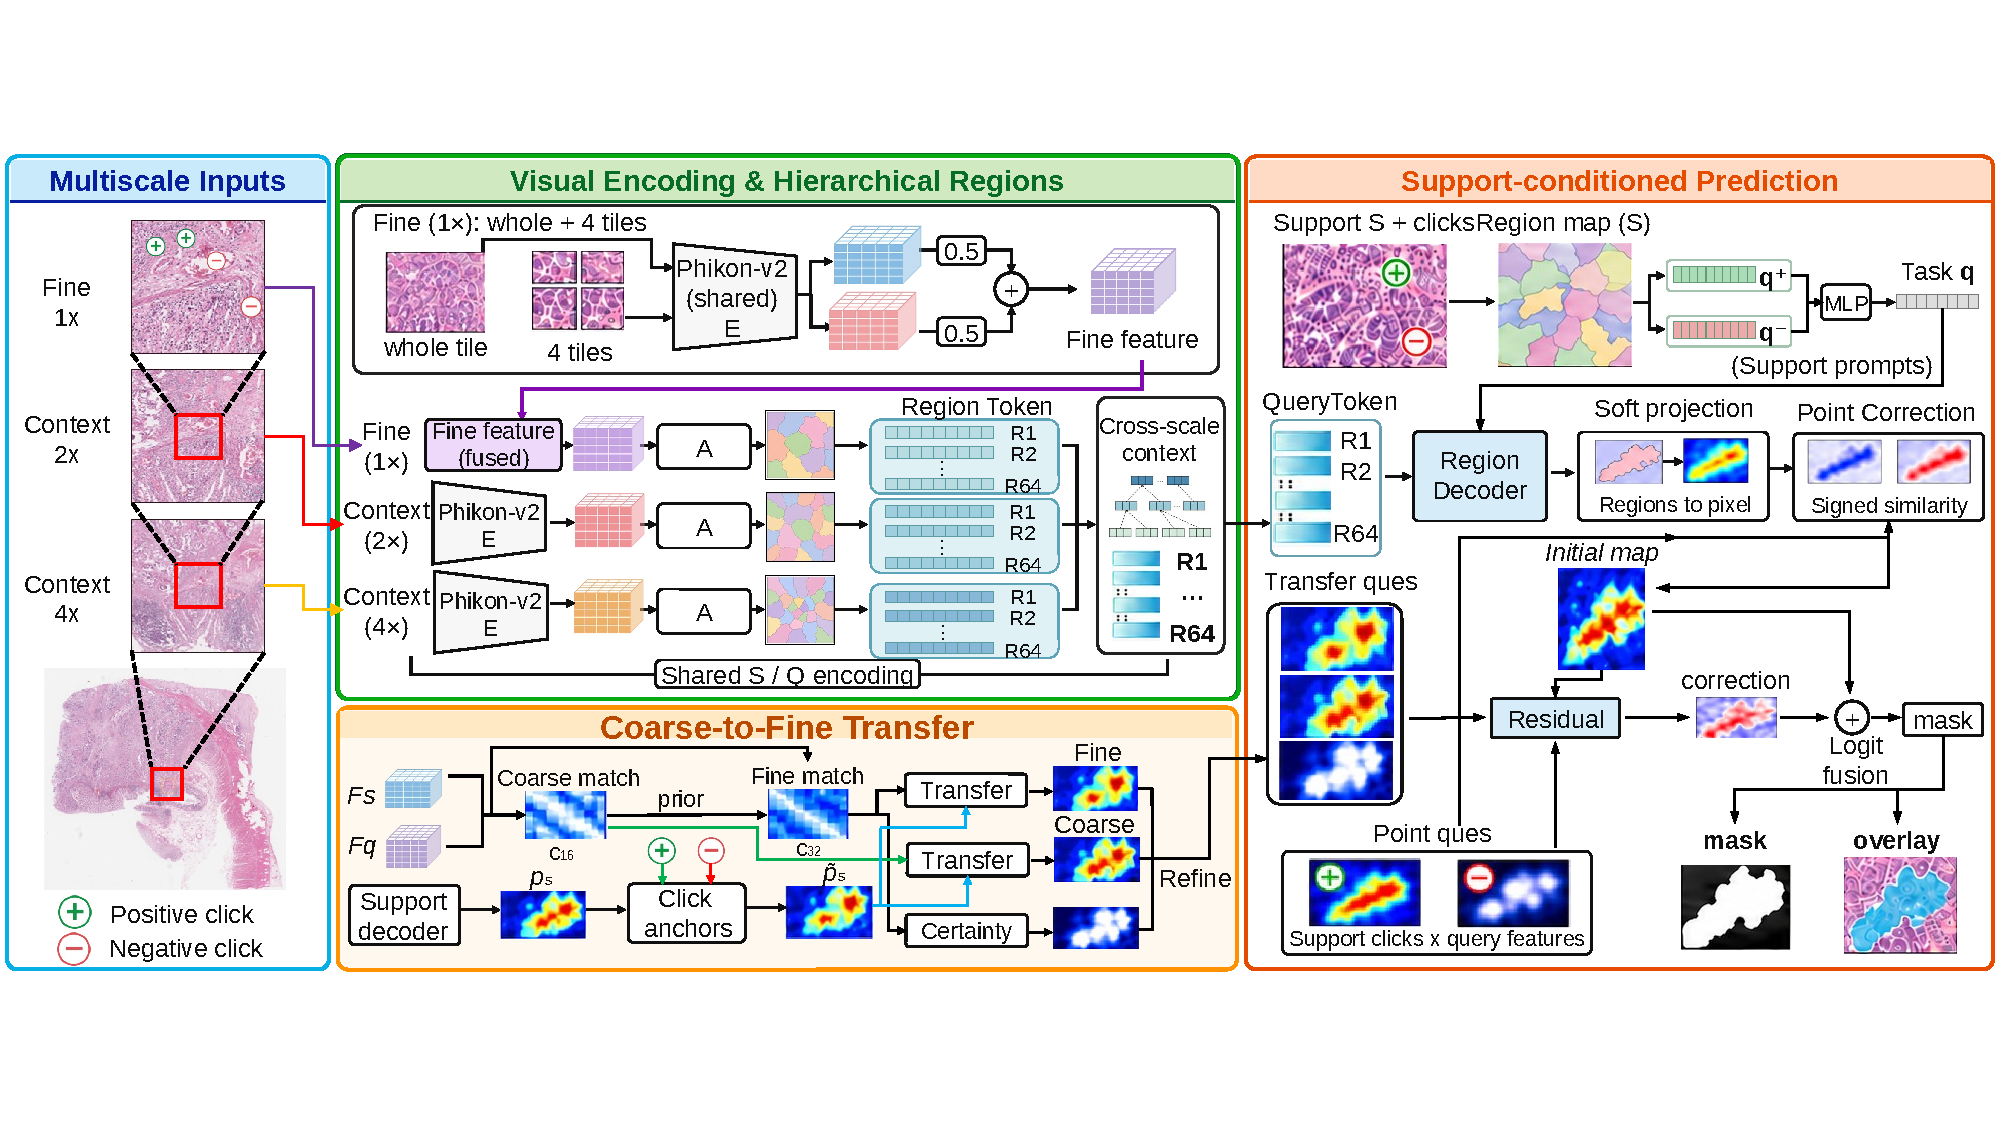
\includegraphics[width=\textwidth,trim=0 72bp 0 72bp,clip]{figures/method.pdf}
\caption{FewClick同片支持—查询分割框架。共享且冻结的Phikon-v2特征结合$1\times$、$2\times$和$4\times$视野，并对整块与分块精细特征取平均。软分配$A$池化区域token，用于跨尺度上下文交互。正负支持点击生成提示汇总向量$q^+/q^-$和任务向量$q$，用于查询区域解码。软投影与正负点相似度修正得到$p_0$。相同路径预测支持概率，并在迁移前通过点击进行锚定。投影特征$F_S/F_Q$构成粗尺度及先验引导的细尺度对应$C_{16}/C_{32}$；下标表示网格尺寸。迁移概率、基于熵的确定性、初始预测及点线索共同输入有界残差头。上采样后的修正量加至初始\emph{logits}，随后通过sigmoid并以$0.5$为阈值生成掩码。远端查询不接收人工点击。组织示例与中间特征图仅作示意。}
\label{fig:overview}
\end{figure*}
FewClick通过正负支持条件建模与密集概率迁移，将点击定义的组织目标传播至同一切片的各区域，并利用多尺度区域上下文组织空间证据（图~\ref{fig:overview}）。

\subsection{由提示定义的组织分割}
每次交互定义一个目标与其余组织之间的二分类任务。设$W$为一张WSI，$S$为支持图像块，$\mathcal P^+$和$\mathcal P^-$分别为其正负点击集合，$Q$为查询图像块。模型预测为
\begin{equation}
 p_Q=f_\theta(Q\mid S,\mathcal P^+,\mathcal P^-).
\end{equation}
支持图像块与远端查询图像块位于同一切片的不同物理位置。远端图像块评价要求二者的最大输入覆盖范围互不相交。更换切片或目标时，使用新的支持示例。训练使用支持与查询标注；推理仅使用二者的图像及支持点击。

\subsection{整块与分块特征融合}
\label{sec:fusion}
组织结构与精细构造需要不同的采样密度。对于每个支持或查询位置，我们提取同心的精细视野以及$2\times$、$4\times$物理视野，并将其分别缩放至$512\times512$。所有视野共享一个冻结的公开Phikon-v2骨干网络。

精细视野包含两条编码路径。一条编码完整图像块；另一条将其划分为四个互不重叠的$256\times256$分块，将各分块缩放至$512\times512$，并编码为原生$32\times32$空间token。将四个网格拼接后，在$64\times64$分辨率上恢复其空间排列。我们将整块网格对齐至这一分辨率，并融合两种表征：
\begin{equation}
 E_f=\tfrac12\operatorname{Align}(F_{\rm whole})
     +\tfrac12\operatorname{Stitch}(F_1,F_2,F_3,F_4).
\label{eq:fusion}
\end{equation}
更大的视野提供区域上下文。每个位置需要七次骨干网络编码：一次完整精细图像块编码、四次分块编码和两次上下文视野编码。

\subsection{提示条件下的区域层级}
\label{sec:regions}
\paragraph{空间上下文池化。}
每个视野在$64\times64$特征网格上构建$64$个$256$维区域token。令$F_s(x)$表示尺度$s\in\{f,m,c\}$上的投影特征，$a_s(x,k)$表示分配头的输出。区域$k$在规则$8\times8$网格上具有锚点$c_k$。位置$u(x)$与锚点$c_k$均位于$[-1,1]^2$，其软分配和池化token为
\begin{align}
 A_s(x,k)&=\operatorname{softmax}_{k}\!\left(a_s(x,k)-\frac{\|u(x)-c_k\|^2}{0.08}\right),\label{eq:assignment}\\
 r_{s,k}&=\frac{\sum_x A_s(x,k)F_s(x)}{\max(\sum_x A_s(x,k),10^{-6})}.
\end{align}
分配头以零初始化，并由分割监督更新。共享融合映射利用图像特征处理这些token；辅助细胞上下文与计数输入均固定为零。分配正则项对各视野的分配总量均衡、熵与紧致性项取平均，其权重分别为$0.01$、$0.001$和$0.01$。

\paragraph{跨尺度上下文。}
相邻尺度间的连接由物理重叠关系定义。我们将子视野映射至父视野的中央区域，累计二者分配图之间的重叠乘积，并为每个子区域保留至多四个有效父区域。此离散建边过程不参与计算图求导。稀疏的自底向上注意力依次更新中间尺度和粗尺度token。精细尺度token接收来自父区域及祖先区域的自顶向下注意力残差，并由一个零初始化可学习标量的双曲正切值进行门控。区域中心和面积均在共同的$4\times$坐标系中表示。

\paragraph{正负提示编码。}
我们在每个支持点击处对精细尺度分配图进行插值，并池化对应的区域token。集合编码时，归一化token结合位置、正负符号及可学习尺度嵌入，其中尺度索引固定。点击坐标位于$[0,1]^2$。共享的两层、四头集合编码器~\cite{lee2019settransformer}和可学习查询池化分别将正负集合汇总为$q^+$与$q^-$。二者的对比关系定义任务token：
\begin{equation}
 q=\operatorname{MLP}([q^+,q^-,q^+-q^-]).
\end{equation}

\paragraph{区域解码与像素投影。}
$192$个区域节点接收尺度嵌入。查询节点对带有位置和正负符号嵌入的支持提示token执行交叉注意力，并融合任务、几何及正负余弦相似度信息。图解码器保留包含自连接的尺度内六近邻连接与相邻尺度间的双向边。二分类头预测精细区域logits $o_k$。经上采样和归一化的分配将区域概率投影至像素：
\begin{equation}
 p_r(x)=\sum_k\bar A_f(x,k)\,\sigma(o_k).
\label{eq:projection}
\end{equation}
我们将该概率截断至$[10^{-6},1-10^{-6}]$，再转换为像素logits。相同的支持条件路径也用于预测支持掩码。

\subsection{正负点相似度修正}
\label{sec:point}
区域编码上下文，而点击位置提供直接的外观示例。共享$1\times1$投影将精细支持与查询特征从$256$维映射至$64$维。我们在点击处采样支持特征，并计算它们与归一化查询特征之间的余弦相似度。

正负点击各自的最大与平均相似度、正负最大相似度之差、缩放至$64\times64$的区域概率$p_r$及其不确定性$4p_r(1-p_r)$组成七个输入通道。卷积头预测修正量，经上采样后加至区域预测得到的logits。其最后一层以零初始化。此路径同时生成初始查询概率$p_0$与支持概率$p_S$。

\subsection{由粗到细的密集概率迁移}
\label{sec:transfer}
我们通过密集支持—查询对应关系迁移预测的支持概率场。

\paragraph{由点击锚定的支持概率。}
令$\bar p_S=\operatorname{Resize}_{32}(\operatorname{stopgrad}(p_S))$。正负点击场$g^+$与$g^-$分别累加同符号点击处的单位峰值高斯函数，其在$[0,1]^2$坐标中的标准差为$1/32$。锚定后的概率为
\begin{equation}
 \widetilde p_S=\frac{\bar p_S+4g^+}{1+4g^++4g^-}.
\label{eq:anchor}
\end{equation}
这会在点击附近约束待迁移的支持证据。

\paragraph{由粗到细的对应关系。}
平均池化将投影后的$64\times64$特征转换为$32\times32$和$16\times16$网格。特征归一化后，查询—支持余弦相似度形成矩阵$K_{32}$与$K_{16}$。以温度$\tau=0.1$沿支持位置进行softmax，得到粗尺度对应$C_{16}$。扩展$\mathcal U$将每个粗尺度查询行复制至四个子位置，并将每个支持位置的概率质量均分给四个子位置。令$\Pi_{32}=\max(\mathcal U(C_{16}),10^{-8})$，则有
\begin{align}
 C_{16}&=\operatorname{softmax}_{S}(K_{16}/\tau),\\
 C_{32}&=\operatorname{softmax}_{S}\!\left(K_{32}/\tau
                  +0.5\log \Pi_{32}\right).
\label{eq:correspondence}
\end{align}
矩阵的行与列分别索引查询和支持位置；$C_{16}$与$C_{32}$的尺寸分别为$256\times256$与$1024\times1024$。

\paragraph{迁移与残差细化。}
将概率网格展平为向量后，对应关系迁移锚定后的概率场（$\operatorname{Pool}$为$2\times2$平均池化）：
\begin{equation}
 t_{32}=C_{32}\widetilde p_S,\qquad
 t_{16}=C_{16}\operatorname{Pool}(\widetilde p_S).
\end{equation}
迁移后的向量恢复为空间网格。匹配确定性为一减去$C_{32}$各行的熵与$\log 1024$之比。精细迁移、缩放后的粗尺度迁移、确定性、$p_0$、$4p_0(1-p_0)$、正负最大相似度及其差值在$32\times32$网格上组成八通道输入$z_Q$。一个$3\times3$卷积、GELU及一个$1\times1$卷积预测有界logit残差：
\begin{equation}
 p_Q=\sigma\!\left(\operatorname{logit}(p_0)
                +\operatorname{Up}[2\tanh h(z_Q)]\right).
\label{eq:residual}
\end{equation}
上采样将输出恢复至$512\times512$分辨率。密集迁移用于远端任务；本图交互使用区域和点修正路径。完整模型保留点击锚定与粗尺度先验。

\subsection{训练目标与优化}
\label{sec:training}
训练涵盖本图交互、同片目标存在迁移与目标缺失迁移。固定队列包含$9{,}500$个任务：$4{,}000$个本图任务、$5{,}000$个远端目标存在任务和$500$个远端目标缺失任务。每次更新累计四个任务，共进行$2{,}375$次更新。目标函数为
\begin{equation}
 \mathcal L=\mathcal L_Q+0.25\,\mathbf{1}_{\rm remote}\mathcal L_S
                  +0.1\mathcal L_{\rm click}+\mathcal L_{\rm assign}.
\end{equation}
分割损失结合有效像素上的二元交叉熵、用于目标存在任务的soft Dice，以及权重为$0.5$的边界带交叉熵。对于目标缺失查询，使用平均预测概率的$0.1$倍替代Dice项。当正负标签均存在时，交叉熵对正负像素损失等权平均。点击损失约束正负提示处的支持预测。远端任务的$\mathcal L_{\rm assign}$对支持和查询图像取平均。

我们使用AdamW，学习率与权重衰减均为$10^{-4}$。公开骨干网络保持冻结，下游模块重新初始化。功能检查使用训练数据，正式训练前再次重新初始化下游模块。推理使用最后一次更新后的模型，并固定概率阈值为$0.5$。

\subsection{基于单个支持集的整片推理}
\label{sec:wsi}
每个“切片—目标”组合使用一个支持图像块及其正负点击。查询窗口复用该支持状态；更换切片或目标时重新设置。设支持精细视野尺寸为$(b_w,b_h)$，查询网格使用$\lfloor b_w/2\rfloor$与$\lfloor b_h/2\rfloor$的步长。通过与边缘对齐的窗口补全最后一行和最后一列，并将支持位置纳入网格。上下文视野保持同心，图像外部使用白色填充。

每个窗口的概率通过像素中心对齐的双线性插值映射至标注网格。在重叠位置，对所有覆盖窗口取平均：
\begin{equation}
 p_W(x)=\frac{\sum_j\mathbf{1}[x\in\Omega_j]p_j(x)}
                   {\sum_j\mathbf{1}[x\in\Omega_j]},\qquad
 M_W(x)=\mathbf{1}[p_W(x)\geq0.5].
\end{equation}
每个输出像素必须至少获得一次预测贡献。整片Dice对每个有效标注像素仅计数一次。严格远端评价移除所有受影响窗口的精细输出矩形之并集；受影响窗口指其$4\times$输入覆盖范围与支持区域的$4\times$输入覆盖范围相交的窗口。在读取标注进行评分之前，预测已固定；未标注像素不参与评价。

\section{实验}
\label{sec:experiments}
\subsection{数据与评价设置}
我们使用CRC和TIGER组织数据。训练集与开发集按空间块划分，支持—查询对以及不同划分之间均保持完整$4\times$输入覆盖范围的分离，并保留患者及切片来源信息。

远端开发队列使用$300$个CRC支持图像块，以及来自$75$张查询切片的$3{,}200$个不同查询图像块，覆盖表~\ref{tab:wsi_tissue}中的11种组织；背景提供有效负类像素。在$11{,}000$个任务中，$7{,}334$个包含目标，$3{,}666$个不含目标。每个任务使用三个正支持点击与两个负支持点击，依据固定规则从支持标注模拟生成，并在各方法间共享。该远端队列用于方法比较与选择。整片评价使用15张切片、152个组织任务。用于整片测试的患者病例均未出现在训练集或开发集中。

\subsection{比较方法与评价指标}
\label{sec:baselines}
我们将FewClick与SANSA、SAM、SAM2、WSI-SAM和SAM-Med2D比较。各方法使用相同的$9{,}500$个新增目标域训练任务、$2{,}375$次更新及支持点击，并使用最终权重进行评价。公开预训练、模型架构、输入视野和适配模块遵循各方法的配置。匹配的量为新增目标域数据适配预算。

SANSA适配其公开Universal adapter，实现支持到查询的传播。SAM系列模型使用由支持信息调节的迁移桥生成自动密集提示；WSI-SAM还使用固定规则生成的稀疏提示。图像编码器均冻结。SANSA使用单个精细视野；SAM、SAM2与SAM-Med2D使用三个对齐视野，WSI-SAM使用精细与$2\times$视野。FewClick与SANSA分别训练7.03M和26.33M个参数。完整的初始化与适配配置见补充材料。

我们报告目标存在查询的类别宏平均Dice，以及目标缺失查询的误报面积比例（FPA）。小目标与大目标分别占有效查询面积的$<20\%$和$\geq20\%$。精确率、召回率以及物理容差为$2\,\mu$m的边界F1用于刻画覆盖与轮廓质量。对于WSI，先在不重复的有效像素上计算每个“切片—目标”组合的Dice，再对各组织内的切片取平均，最后对11种组织等权平均。整片与严格远端评分域遵循第~\ref{sec:wsi}节的定义。

\subsection{同片远端图像块分割}
\begin{table}[t]
\centering
\caption{在11,000个任务上的同片远端分割结果。各任务使用三个正支持点击和两个负支持点击，查询区域无点击。Dice与大目标列分别报告目标存在Dice和大目标Dice。所有指标均为百分比；粗体表示最优值。}
\label{tab:remote}
\small
\setlength{\tabcolsep}{4pt}
\begin{tabular}{@{}lrrr@{}}
\toprule
方法 & Dice $\uparrow$ & 大目标 $\uparrow$ & FPA $\downarrow$ \\
\midrule
SAM & 30.31 & 64.40 & 27.01 \\
SAM2 & 33.60 & 66.50 & 18.91 \\
WSI-SAM & 23.81 & 50.02 & 23.43 \\
SAM-Med2D & 24.28 & 54.80 & 39.87 \\
SANSA & 41.54 & 77.22 & 14.79 \\
FewClick & \textbf{42.11} & \textbf{78.49} & \textbf{7.75} \\
\bottomrule
\end{tabular}
\end{table}

表~\ref{tab:remote}比较了六种方法在相同任务上的表现。FewClick的目标存在宏平均Dice为42.11\%，大目标Dice为78.49\%，目标缺失FPA为7.75\%。SANSA的对应指标分别为41.54\%、77.22\%和14.79\%。FewClick的两项Dice分别提高0.57和1.27个百分点，FPA降低7.04个百分点，相对下降47.6\%。

对75张查询切片进行4,000次配对重采样后，FPA差值的95\%区间为$[-8.37,-5.70]$个百分点，目标存在Dice差值的区间为$[-0.11,1.31]$。FPA区间完全低于零，Dice区间包含零。

\subsection{整片分割}
\begin{table}[t]
\centering
\caption{在15张切片、152个组织任务上的整片类别宏平均Dice（\%）。每个“切片—目标”组合使用一个支持图像块以及三个正点击和两个负点击。严格远端评价排除输入覆盖范围与支持区域相交的相关输出。}
\label{tab:wsi}
\small
\setlength{\tabcolsep}{4pt}
\begin{tabular}{@{}lrr@{}}
\toprule
方法 & 整片 $\uparrow$ & 严格远端 $\uparrow$ \\
\midrule
SAM & 18.86 & 16.63 \\
SAM2 & 23.58 & 21.01 \\
WSI-SAM & 15.85 & 14.25 \\
SAM-Med2D & 13.59 & 11.97 \\
SANSA & 33.23 & 30.12 \\
FewClick & \textbf{43.75} & \textbf{40.98} \\
\bottomrule
\end{tabular}
\end{table}

\begin{table*}[t]
\centering
\caption{六种方法在相同15张WSI上的逐组织整片Dice（\%）。每种组织的得分对有效“切片—目标”组合取平均；$n$为参与该组织评价的切片数。宏平均对11种组织等权计入。粗体表示每行最高的Dice。}
\label{tab:wsi_tissue}
\small
\setlength{\tabcolsep}{0.5pt}
\begin{tabularx}{\textwidth}{@{}p{0.20\textwidth}*{7}{>{\centering\arraybackslash}X}@{}}
\toprule
组织 & $n$ & SAM & SAM2 & WSI-SAM & SAM-Med2D & SANSA & FewClick \\
\midrule
肿瘤上皮 & 15 & 50.02 & 58.79 & 35.53 & 36.87 & 78.97 & \textbf{79.17} \\
肿瘤间质 & 15 & 31.53 & 36.39 & 27.11 & 22.86 & 42.97 & \textbf{55.23} \\
坏死 & 15 & 15.09 & 20.29 & 14.83 & 11.72 & 32.91 & \textbf{44.10} \\
正常腺体 & 15 & 18.35 & 24.27 & 17.41 & 8.77 & 26.10 & \textbf{43.23} \\
正常间质 & 15 & 5.68 & 9.01 & 5.61 & 5.48 & 20.80 & \textbf{25.12} \\
黏膜下层／浆膜 & 15 & 22.75 & 25.18 & 19.94 & 19.47 & 36.15 & \textbf{49.83} \\
肌肉 & 15 & 31.82 & 37.27 & 29.46 & 23.50 & 51.27 & \textbf{61.32} \\
淋巴组织聚集 & 7 & 2.17 & 2.61 & 1.51 & 1.96 & 5.46 & \textbf{34.24} \\
黏液 & 15 & 3.82 & 6.92 & 3.79 & 3.05 & 9.23 & \textbf{18.76} \\
脂肪 & 15 & 22.96 & 30.58 & 16.14 & 13.59 & \textbf{49.51} & 48.67 \\
血液 & 10 & 3.22 & 8.10 & 3.01 & 2.25 & 12.13 & \textbf{21.59} \\
\midrule 宏平均 & -- & 18.86 & 23.58 & 15.85 & 13.59 & 33.23 & \textbf{43.75} \\
\bottomrule
\end{tabularx}
\end{table*}

\begin{figure*}[t]
\centering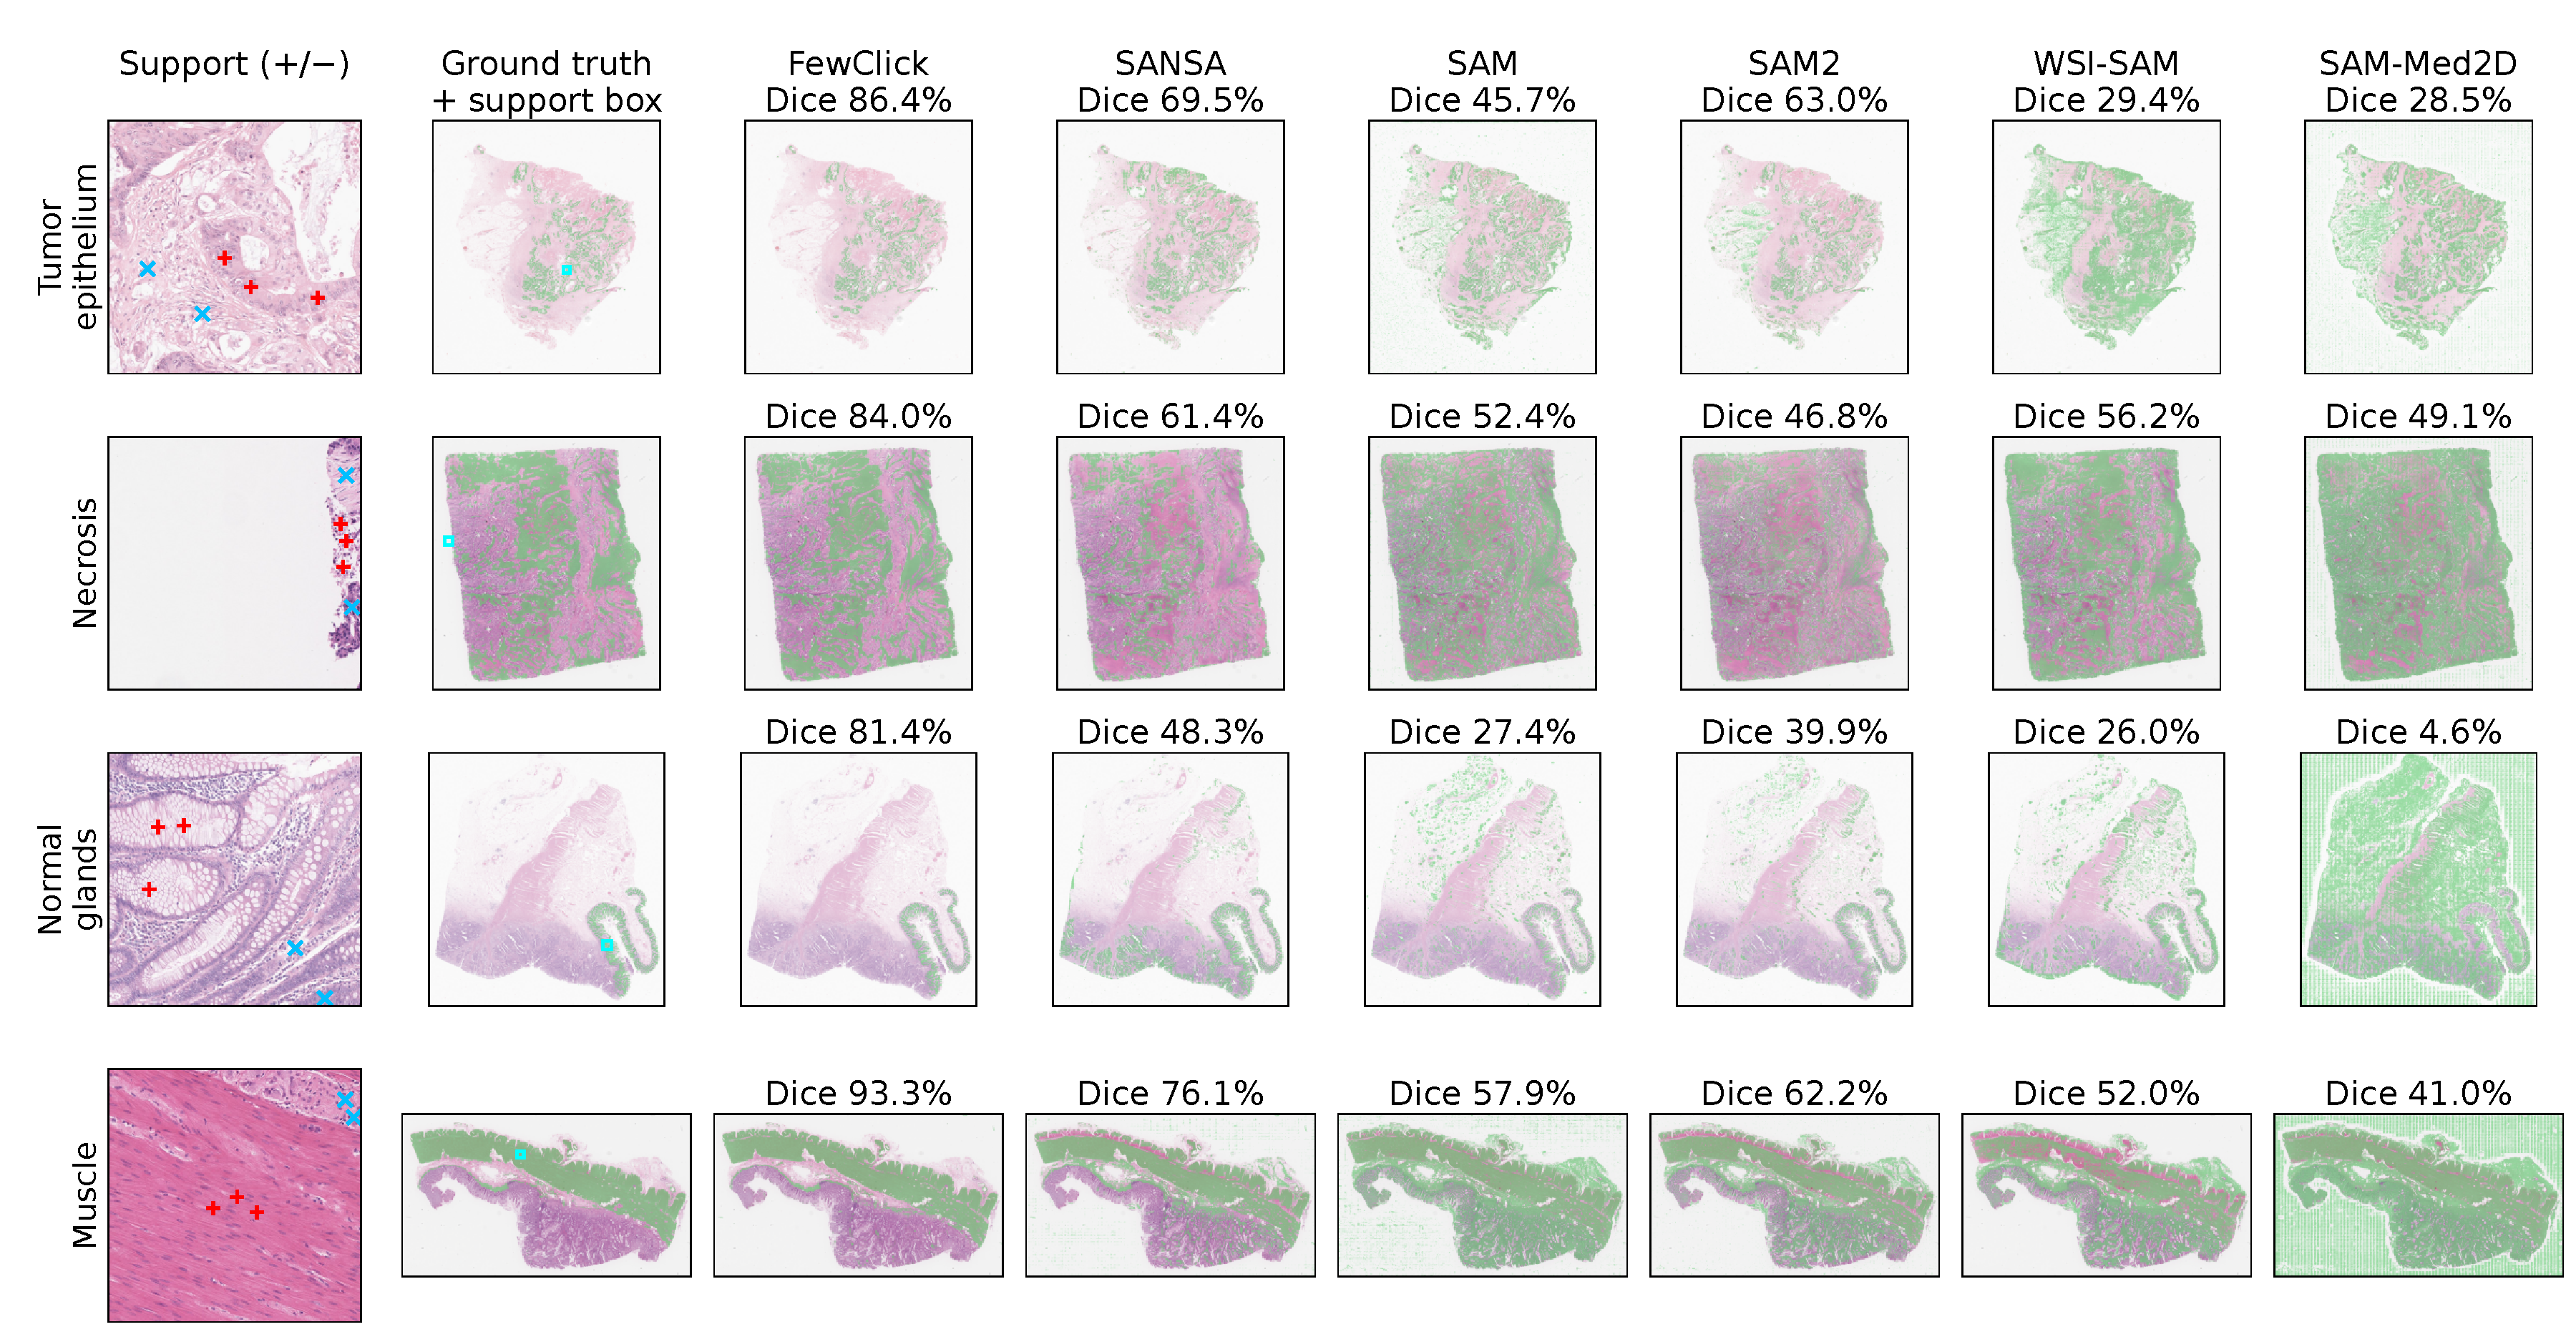
\includegraphics[width=\textwidth]{figures/figure2.pdf}
\caption{选取的整片分割案例，每个案例使用一个支持集。各行依次为肿瘤上皮、坏死、正常腺体和肌层；各列为支持点击、带支持框的真实标注及六种方法的预测。红色加号与天蓝色叉号分别表示正负点击。绿色覆盖表示目标组织，青色框标示支持图像块。面板分数为相应“切片—目标”组合的整片Dice，基于原始分辨率的有效像素计算。}
\label{fig:wsi}
\end{figure*}
六种方法在15张WSI上完成了912次“组织—方法”评价。FewClick的整片宏平均Dice为43.75\%，严格远端宏平均Dice为40.98\%，分别比SANSA的33.23\%与30.12\%高10.52和10.86个百分点（表~\ref{tab:wsi}）。排除输入覆盖范围与支持区域相交的相关输出后，增益仍然存在。对每张切片内可评价的组织取平均后，FewClick在两个评分域上均优于SANSA，覆盖15张切片中的14张。以切片为聚类单位的配对Bootstrap给出整片与严格远端增益的95\%置信区间，分别为$[7.62,13.56]$和$[8.02,13.87]$个百分点。

在11种组织中的10种上，FewClick的整片Dice高于SANSA；脂肪组织略低。正常腺体与淋巴组织聚集分别提高17.13和28.78个百分点（表~\ref{tab:wsi_tissue}）。二者在严格远端域上的增益仍为18.04和29.11个百分点，支持了超出支持邻域的迁移能力。图~\ref{fig:wsi}展示了选取的组织案例。

\paragraph{从窗口到整张切片。}
在正式评价的前三张WSI上（32个“切片—目标”组合），FewClick与SANSA的目标存在窗口Dice分别为37.79\%和37.37\%；融合后的整片Dice为45.65/34.85\%。将每个像素分配给覆盖它且中心最近的窗口，不进行重叠平均时，整片Dice为46.41/34.70\%。因此，整片增益在重叠平均之前就已存在。目标存在窗口Dice仅对含有目标的窗口取平均，而整片Dice对每个有效像素计数一次，并包含目标缺失窗口中的误报。在这些窗口中，FewClick/SANSA的FPA为3.26/8.31\%。较低的目标缺失窗口FPA有助于形成更大的整片增益；该指标同时反映目标覆盖与对非目标区域的排除。

\begin{figure*}[t]
\centering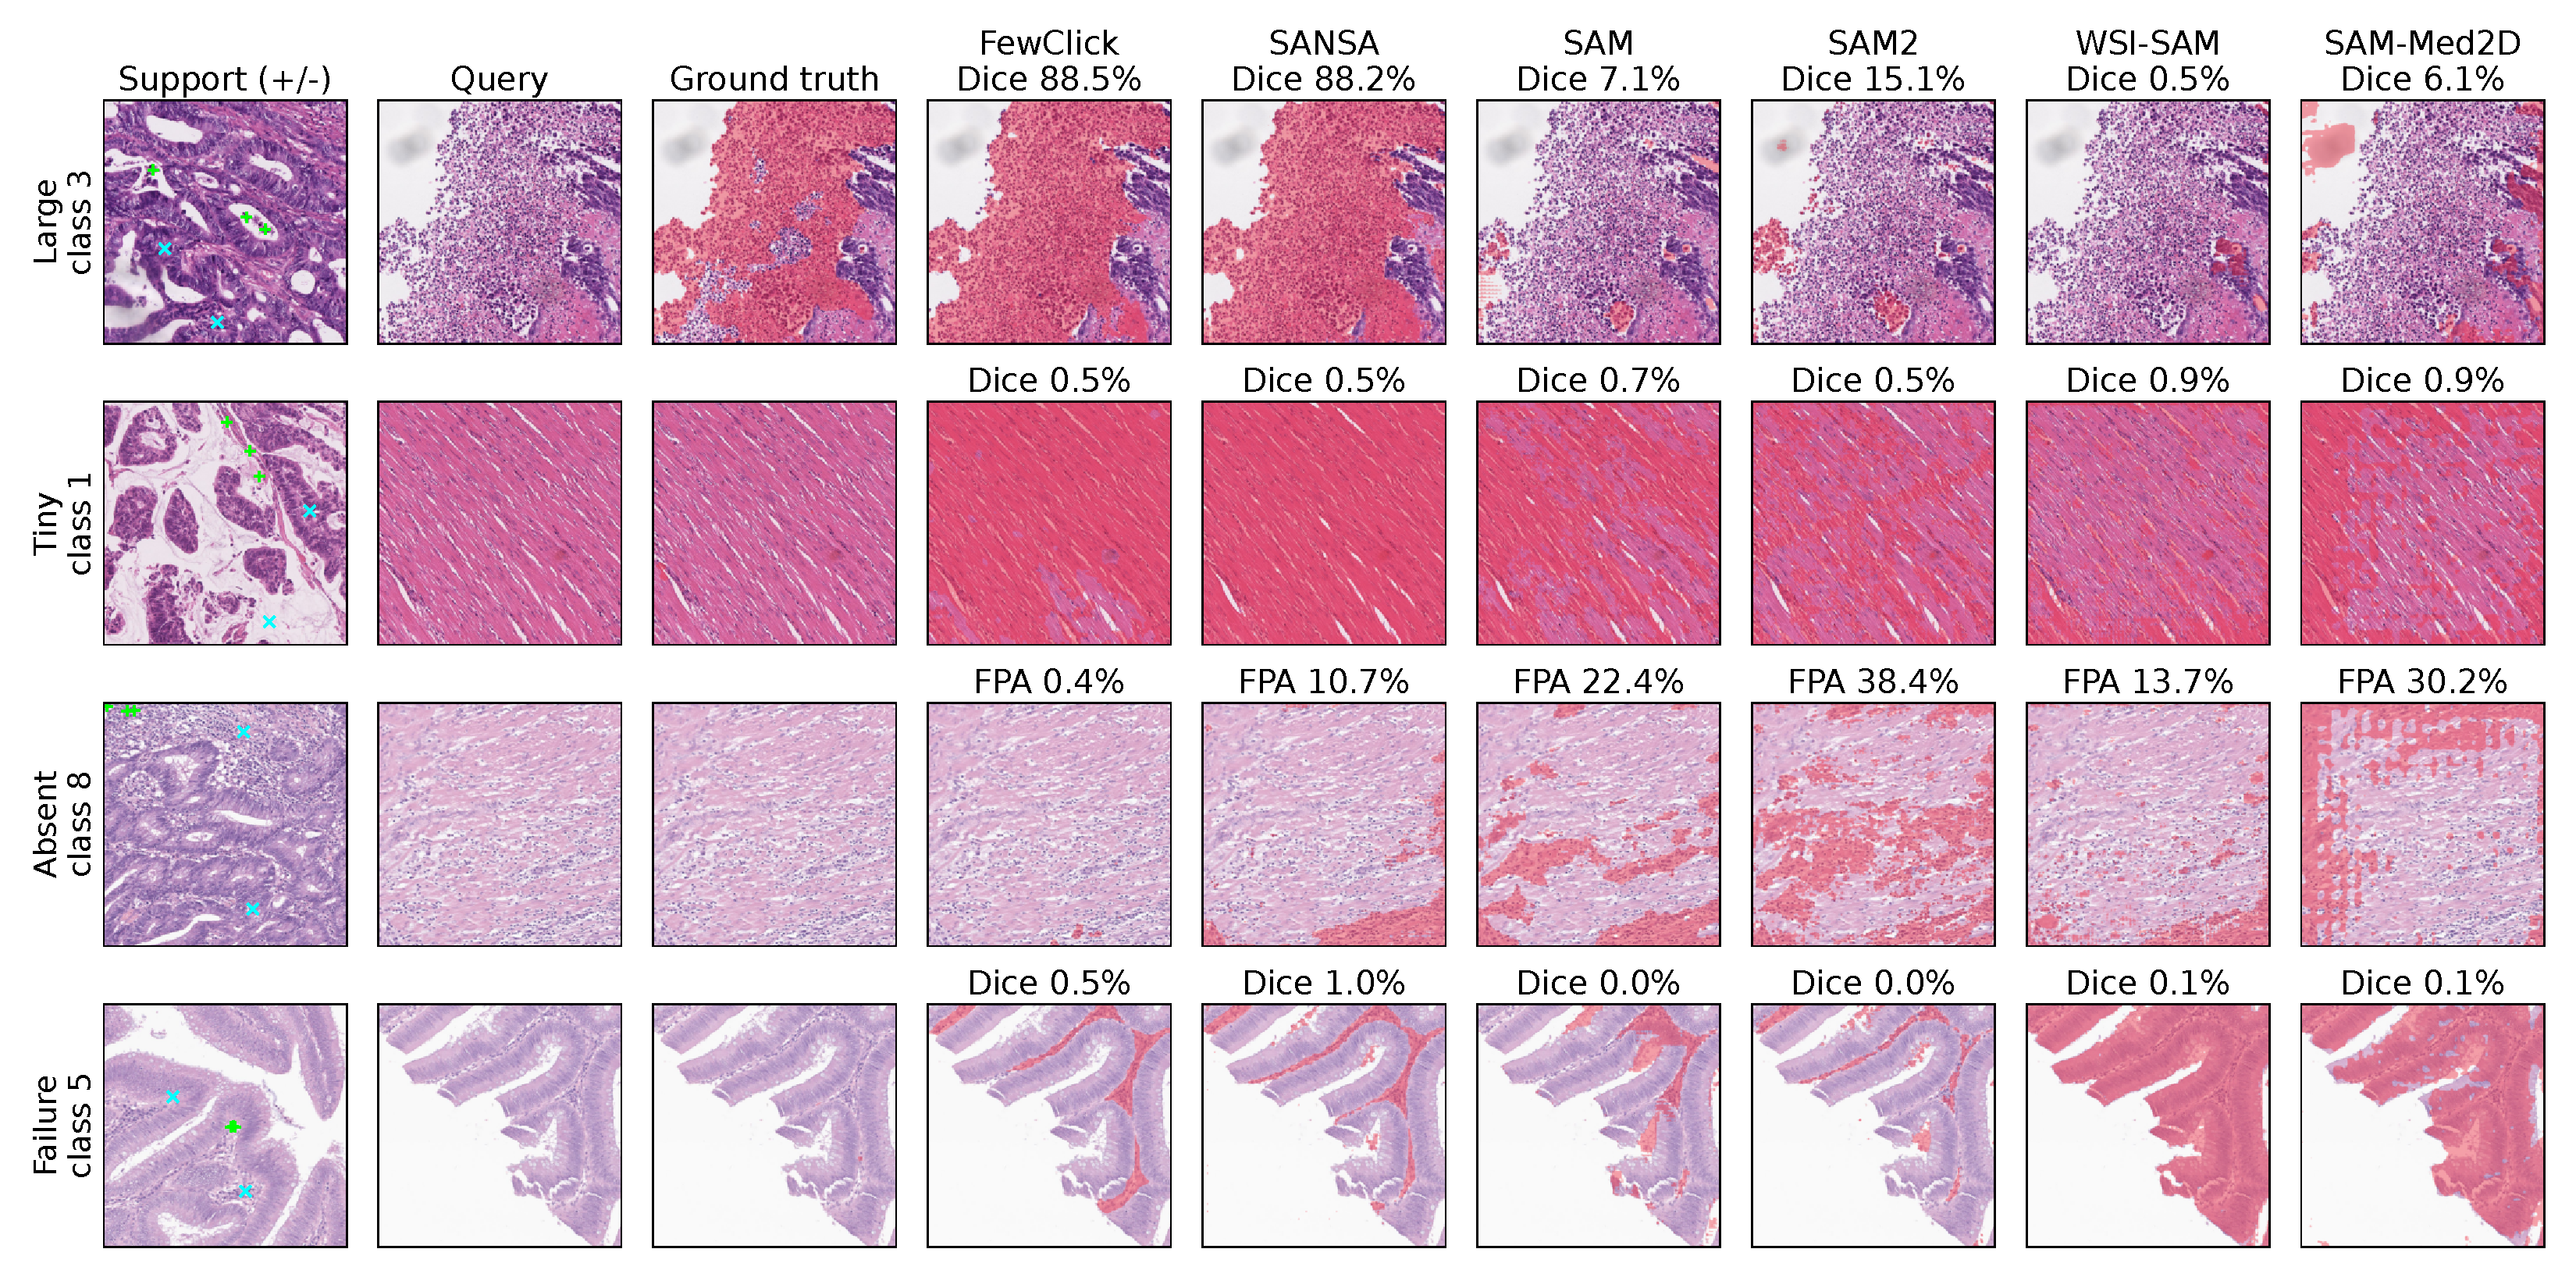
\includegraphics[width=\textwidth]{figures/figure3.pdf}
\caption{远端定性案例：大目标、微小目标、目标缺失及低Dice失败案例。每行包含支持点击、查询图像、真实标注及六种方法的预测。案例选取各组中最接近FewClick Dice中位数（目标存在）或FPA中位数（目标缺失）的任务，并以任务索引打破并列。绿色加号与青色叉号分别表示正负支持点击；红色覆盖表示目标组织。目标存在案例的面板分数为任务级Dice，目标缺失案例为FPA。指标基于原始$512\times512$预测计算。}
\label{fig:failures}
\end{figure*}

\subsection{结构消融}
\begin{table}[t]
\centering
\caption{匹配条件下的结构消融：(a) 精细表征与密集迁移；(b) 融合模型的组件。P/L/S分别表示目标存在、大目标和小目标Dice；所有数值均为百分比。Dice越高越好，FPA越低越好。}
\label{tab:ablation}
\small
\setlength{\tabcolsep}{4pt}
\textbf{(a) 精细表征 $\times$ 密集迁移}\\[2pt]
\begin{tabular}{@{}llrrr@{}}
\toprule
精细视野 & 迁移 & P & L & FPA \\
\midrule
整块 & 否 & 39.19 & 73.81 & 6.71 \\
整块 & 是 & 39.97 & 76.51 & 8.10 \\
分块 & 否 & 40.16 & 74.63 & 5.74 \\
分块 & 是 & 40.87 & 76.84 & 7.04 \\
融合 & 否 & 40.92 & 75.37 & 5.61 \\
融合 & 是 & 42.11 & 78.49 & 7.75 \\
\bottomrule
\end{tabular}
\par\vspace{4pt}
\textbf{(b) 融合模型组件}\\[2pt]
\begin{tabular}{@{}lrrrr@{}}
\toprule
变体 & P & L & S & FPA \\
\midrule
完整FewClick & 42.11 & 78.49 & 28.19 & 7.75 \\
无密集迁移 & 40.92 & 75.37 & 28.04 & 5.61 \\
无区域消息 & 41.66 & 77.66 & 28.09 & 6.90 \\
\bottomrule
\end{tabular}
\end{table}

我们在使用与不使用密集迁移两种条件下，分别训练整块、四分块和等权融合表征，形成$2\times3$组比较。各模型均从相同的公开初始化出发，遵循$9{,}500$个任务／$2{,}375$次更新的预算，并在相同的$11{,}000$个远端任务上评价。

\paragraph{同特征原型基线。}
Proto-MS使用轻量卷积解码器，根据正负点击原型与相似度预测掩码。它与FewClick共享冻结的Phikon-v2、三个物理视野、整块／分块等权融合、七次编码及训练预算。共同子集包含550个小目标、262个大目标及275个目标缺失任务，抽样不使用模型预测。目标存在Dice按各组织在原队列中的大小目标比例加权。在这$1{,}087$个任务上，FewClick的目标存在Dice提高1.49个百分点（42.32\%对40.83\%），大目标Dice提高4.17个百分点（75.67\%对71.50\%）。其目标缺失FPA更高，为6.32\%，Proto-MS为5.16\%。在三张WSI上，融合后的整片Dice从Proto-MS的42.13\%提高至FewClick的45.65\%。这些分割重叠增益在相同预训练特征和输入视野下仍然存在。

\paragraph{密集概率迁移。}
在融合特征下，加入密集迁移使目标存在Dice从40.92\%提高至42.11\%，大目标Dice从75.37\%提高至78.49\%；根据未舍入数值计算的增益分别为1.20和3.13个百分点。小目标Dice从28.04\%提高至28.19\%。FPA从5.61\%上升至7.75\%，说明该组件主要改善较大的目标区域，同时增加了目标缺失时的响应。

\paragraph{整块与分块表征。}
无论是否使用密集迁移，融合表征均获得最高的目标存在Dice和大目标Dice（表~\ref{tab:ablation}a），支持了完整组织结构与局部细节的互补作用。

\paragraph{跨尺度区域消息。}
保持相同视野与七次骨干网络编码，将跨尺度区域消息替换为恒等映射，并移除跨尺度解码器边后，目标存在、大目标和小目标Dice分别为41.66\%、77.66\%和28.09\%，FPA为6.90\%。大目标Dice下降0.83个百分点，小于移除密集迁移后的3.13个百分点降幅。两个组件均提高了分割重叠程度，同时增加目标缺失FPA。

\paragraph{可学习区域与固定区域。}
将可学习分配替换为固定空间软网格并进行匹配重训后，在同一组$1{,}087$个任务上，目标存在Dice为42.04\%，FewClick为42.32\%。可学习分配带来的0.28个百分点增益较小；固定网格的大目标Dice略高（76.02\%对75.67\%），而可学习区域将目标缺失FPA从6.67\%降至6.32\%。

\paragraph{各组件对整片分割的影响。}
在三张WSI上，移除密集迁移使融合后的整片Dice从45.65\%降至41.70\%，移除跨尺度区域消息后则为44.27\%。严格远端Dice呈相同排序：FewClick为43.04\%，移除密集迁移后为39.42\%，移除区域消息后为41.89\%。移除密集迁移带来的更大降幅，与其对大目标图像块Dice的更大影响一致。



\subsection{效率与提示敏感性}
\begin{table}[t]
\centering
\caption{在单张RTX 5880 Ada GPU上测量100个任务得到的平均延迟和缓存大小。首次预测包含读取与编码；改变提示后的预测复用图像特征。缓存大小包括一对支持—查询特征及提示记忆。}
\label{tab:efficiency}
\small
\setlength{\tabcolsep}{4pt}
\begin{tabular}{@{}lrrr@{}}
\toprule
方法 & 首次（ms） & 更新后（ms） & 缓存（MiB） \\
\midrule
FewClick & 1539.2 & 43.0 & 16.39 \\
SANSA & 1226.3 & 39.1 & 212.38 \\
SAM & 1191.8 & 18.0 & 16.00 \\
SAM2 & 1297.9 & 16.3 & 40.00 \\
WSI-SAM & 767.9 & 36.3 & 34.00 \\
SAM-Med2D & 863.9 & 17.7 & 1.00 \\
\bottomrule
\end{tabular}
\end{table}

六种方法在同一张GPU上依次计时，每种方法预热三次后测量100个任务。首次预测包含读取与编码，使用三个正点击和两个负点击；改变提示后的预测复用图像特征，使用一个正点击和一个负点击。计时通过GPU同步进行，不包含模型加载与评分。

FewClick首次预测平均耗时1539.2\,ms，改变提示后为43.0\,ms，SANSA分别为1226.3/39.1\,ms；二者缓存大小分别为16.39和212.38\,MiB（表~\ref{tab:efficiency}）。FewClick的缓存占用减少92.3\%，同时保持43.0\,ms的提示更新耗时。在共享GPU环境下，FewClick处理每张切片的全部目标平均需要98.0分钟，包含查询读取与编码、解码、融合、评分及保存掩码的核验。

在按组织／目标大小分层哈希选出的330个任务上（220个目标存在、110个目标缺失），将提示从三个正点击、两个负点击减少至一个正点击、一个负点击后，FewClick/SANSA的Dice从53.18/52.83\%降至51.14/51.03\%。保持三个正点击时，加入第二个负点击使FewClick的FPA从9.80\%降至8.20\%。在$512\times512$支持网格上，两像素或五像素的径向扰动使Dice变化不超过0.31个百分点。

\subsection{目标大小、边界与失败分析}

在$5{,}204$个小目标任务上，FewClick的宏平均Dice为28.19\%，SANSA为27.65\%。当目标占有效面积不足1\%时，两者的Dice均低于8\%（7.68/7.59\%）。在$1$--$5\%$与$5$--$20\%$两个面积层中，FewClick/SANSA的Dice分别升至36.98/35.59\%与59.43/59.05\%。

FewClick的总体精确率为39.67\%，高于SANSA的38.21\%；召回率为67.90\%，SANSA为77.75\%；边界F1为25.86\%，SANSA为29.25\%。对于大目标，FewClick同时提高了精确率（77.69\%对76.65\%）与召回率（83.66\%对82.98\%），但边界F1较低（40.35\%对45.51\%）。其更强的大区域覆盖能力因而与较低的精细轮廓准确性并存。

图~\ref{fig:failures}展示了大目标、微小目标、目标缺失和低Dice案例。在目标缺失示例中，FewClick/SANSA的FPA为0.40/10.67\%。在目标面积占比为0.24\%时，FewClick的Dice为0.51\%，同时出现较大范围的非目标响应。

\section{讨论与结论}
FewClick通过一个支持图像块中的少量正负点击，将用户指定的组织传播至整张WSI。在15张WSI、152个组织任务上，整片与严格远端宏平均Dice分别达到43.75\%和40.98\%，比SANSA高10.52和10.86个百分点。在远端开发队列上，目标缺失FPA降低7.04个百分点，同时保持相当的目标存在Dice。

消融实验揭示了覆盖–误检权衡：密集迁移使大目标Dice提高3.13个百分点，同时使目标缺失FPA从5.61\%升至7.75\%。多尺度特征与区域上下文为这一传播流程提供支持。复用缓存时，提示更新耗时43.0\,ms。微小目标与精细轮廓仍具有挑战：目标面积不足1\%时，Dice为7.68\%，总体边界F1为25.86\%。

未来工作将探索更高分辨率的细化与目标尺寸感知训练，以改善微小目标分割和精细边界，同时评估目标缺失区域的误报，并保持同片传播、查询区域无需额外人工提示的设定。

\label{page:main-end}
\clearpage
\section*{LLM Usage Statement}
本研究迭代使用OpenAI ChatGPT/Codex辅助方法与实验规划，训练及评估脚本的实现、调试和运行，结果分析与文献核查，图表制作，以及论文起草、修改和中英文翻译。辅助工作包括在作者指导下生成和修改代码与文本。作者对科学论断、实验结果、参考文献及最终内容负责。

{\small\bibliographystyle{ieeenat_fullname}\bibliography{references}}
\end{document}
